%%=====================================================================================
%%
%%          ToDo :  !!! important !!! on debian based systems you have to install
%%                  biber with sudo apt-get install biber for the bibliography or use 
%%                  bibtex instead but biber/biblatex has utf8 support per default
%%       Filename:  main.tex
%%
%%    Description:  ESK Lab Thesis Template  
%%
%%        Version:  1.0
%%        Created:  25.08.2015
%%       Revision:  none
%%
%%         Author:  B.Eng. Oliver Kehret, okehret@stud.hs-offenburg.de
%%   Organization:  HS Offenburg, Offenburg, Germany
%%      Copyright:  Copyright (c) 2015, B.Eng. Oliver Kehret
%%
%%          Notes:  Inspired by Andreas Walz, Tobias Neff and Karl Voith
%%                
%%=====================================================================================
%---------------------------------------------------------------------------------------------------
% Settings
%---------------------------------------------------------------------------------------------------
\newcommand{\mypapersize}{A4}
\newcommand{\mylaterality}{oneside}
%% "oneside" or "twoside"
\newcommand{\mydraft}{false}
%% "true" or "false"
\newcommand{\myparskip}{half}
%% e.g., "no", "full", "half", ...
\newcommand{\myBCOR}{10mm}
\newcommand{\myfontsize}{11pt}   
\newcommand{\mylinespread}{onehalfspacing} 
%% e.g.onehalfspacing, doublespacing, singlespacing
%% Line spacing in %/100. For example 1.5 means 150% of the usual line
%% spacing. Please use with caution: 100% ("1.0") is fine because the
%% font was designed for it.
\newcommand{\mylanguage}{ngerman,american}
%% NOTE: The *last* language is the active one!
%% BibLaTeX-settings: (see biblatex reference for further description)
\newcommand{\mybiblatexstyle}{numeric}
%% e.g., "alphabetic", "authoryear", ...
%% The biblatex style which is being used for referencing. See
%% biblatex documentation for further details and more values.
%%
%% CAUTION: if you change the style, please check for (in)compatible
%%          "biblatex" package options in the file
%%          "template/preamble.tex"! For example: "alphabetic" does
%%          not have an option "dashed=..." and causes an error if it
%%          does not get removed from the list of options.

\newcommand{\mybiblatexdashed}{false}  %% "true" or "false"
%% If true: replace recurring reference authors with a dash.

\newcommand{\mybiblatexbackref}{true}  %% "true" or "false"
%% If true: create backward links from reference to citations.

\newcommand{\mybiblatexfile}{bib/bibliography.bib}
%% Name of the biblatex file that holds the references.

\newcommand{\mydispositioncolor}{0,0,0}
%% e.g., "30,103,182" (blue/turquois), "0,0,0" (black), ...
%% Color of the headings and so forth in RGB (red,green,blue) values.

\newcommand{\mycolorlinks}{false}  %% "true" or "false"
%% Enables or disables colored links (hyperref package).
\newcommand{\mytodonotesoptions}{disable}
%% e.g., "" (empty), "disable", ...
%% Options for the todonotes-package. If "disable", all todonotes will
%% be hidden (including todos).
%% ========================================================================
%%  Document metadata
%% ========================================================================
%% general metadata:
\newcommand{\myauthor}{Steve Wagner}  %% also used for PDF metadata
% (hyperref)
\newcommand{\myformation}{EI-3nat}
\newcommand{\mytitle}{Bachelor Thesis}  %% also used for PDF metadata (hyperref)
\newcommand{\mysubject}{Extension and Integration of an Abstract Interface to Cryptography Providers}  %% also used for PDF metadata (hyperref)
\newcommand{\mykeywords}{<++keywords++>}  %% also used for PDF metadata (hyperref)
%% this information is used only for generating the title page:
\newcommand{\myworktitle}{Bachelor thesis}  %% official type of work like ``Master theses''
\newcommand{\mygrade}{Bachelor of Engineering} %% title you are getting with this work like ``Master of ...''
\newcommand{\mystudy}{Electronik und Informationstechnik} %% your study like ``Arts''
\newcommand{\myuniversity}{Offenburg University of Applied Sciences} %% your
% university/school
\newcommand{\myinstitute}{Institute of reliable Embedded Systems and
Communication Electronics (ivESK)}
%% affiliation
\newcommand{\myinstitutehead}{Prof. Dr. Axel Sikora} %% head of institute 
\newcommand{\mysupervisor}{Dipl.-Phys. Andreas Walz} %% your supervisor
\newcommand{\myevaluator}{myprof} %% your evaluator
\newcommand{\myhomestreet}{street} %% your home street (with house number)
\newcommand{\myhometown}{town} %% your home town
\newcommand{\myhomepostalnumber}{psn} %% your postal number of home town
\newcommand{\mysubmissionmonth}{month} %% month you are handing in
\newcommand{\mysubmissionyear}{year} %% year you are handing in
\newcommand{\mysubmissiontown}{\myhometown} %% town of handing in (or \myhometown)
%% additional information for generic_documentation title page

%---------------------------------------------------------------------------------------------------
% formating
%---------------------------------------------------------------------------------------------------

\newcommand{\clearemptydoublepage}{\clearpage\newpage\thispagestyle{empty}\cleardoublepage}

\newcommand{\CRule}{\rule{0.95\textwidth}{0.5pt}} % New command to make the lines above figure captions


%---------------------------------------------------------------------------------------------------
% fixme makro
%---------------------------------------------------------------------------------------------------

%\newcommand{\fixme}[1]{\textbf{\large FIXME: #1}}
%\newcommand{\todo}[1]{\textbf{\large TODO: #1}}
%\newcommand{\idea}[1]{\textbf{IDEA: #1 ~\\}}


%---------------------------------------------------------------------------------------------------
% names
%---------------------------------------------------------------------------------------------------

\newcommand{\gci}{Generic Cryptographic Interface (GCI)\xspace}
\newcommand{\embtls}{emb::TLS\xspace}
\newcommand{\tomcrypt}{LibTomCrypt\xspace}
\newcommand{\vaultic}{VaultIC\num{460}\xspace}
\newcommand{\Table}{Table}
\newcommand{\Tables}{Tables}
\newcommand{\Figure}{Figure}
\newcommand{\Figures}{Figures}
\newcommand{\Subfigure}{Subfigure}
\newcommand{\Section}{Section}
\newcommand{\Sections}{Sections}
\newcommand{\Chapter}{Chapter}
\newcommand{\Chapters}{Chapters}
\newcommand{\Equation}{Equation}
\newcommand{\Equations}{Equations}

\newcommand{\Appendix}{Appendix}
\newcommand{\Appendices}{Appendices}
\newcommand{\Ref}{Ref.}
\newcommand{\Refs}{Refs.}

%---------------------------------------------------------------------------------------------------
% units
%---------------------------------------------------------------------------------------------------

\newcommand{\Hz}	{\ensuremath{\mathrm{Hz}}\xspace}
\newcommand{\kHz}	{\ensuremath{\mathrm{kHz}}\xspace}
\newcommand{\MHz}	{\ensuremath{\mathrm{MHz}}\xspace}

\newcommand{\cm}{\ensuremath{\mathrm{cm}}\xspace}
\newcommand{\m}{\ensuremath{\mathrm{m}}\xspace}
\newcommand{\mm}{\ensuremath{\mathrm{mm}}\xspace}
\newcommand{\microm}{\ensuremath{\mu\mathrm{m}}\xspace}
\newcommand{\s}{\ensuremath{\mathrm{s}}\xspace}
\newcommand{\musec}{\ensuremath{\mu\mathrm{s}}\xspace}


%---------------------------------------------------------------------------------------------------
% include figures
%---------------------------------------------------------------------------------------------------
\newcommand{\myfig}[5]{
%% example:
% \myfig{}%% filename in figures folder
%       {width=0.5\textwidth,height=0.5\textheight}%% maximum width/height, aspect ratio will be kept
%       {}%% caption
%       {}%% optional (short) caption for list of figures
%       {}%% label
\begin{figure}%[htp]
  \begin{center}
     \includegraphics[keepaspectratio,#2]{figures/#1}
     \caption[#4]{#3}
     \label{#5} %% NOTE: always label *after* caption!
  \end{center}
  
\end{figure}
}



%% ========================================================================
%%  preamble
%% ========================================================================
%_____________________________________________________________________________________
%
%       Filename:  preamble.tex
%
%    Description:  Thesis Template HS Offenburg
%
%        Version:  1.0
%        Created:  13.11.2015
%       Revision:  none
%
%         Author:  B.Eng. Oliver Kehret, okehret@stud.hs-offenburg.de
%   Organization:  HS Offenburg, Offenburg, Germany
%      Copyright:  Copyright (c) 2015, B.Eng. Oliver Kehret
%
%          Notes:  Inspired by Andreas Walz, Tobias Neff and Karl Voith
%                
%_____________________________________________________________________________________
\documentclass[]{beamer}
\usetheme{Madrid}

%_____________________________________________________________________________________
% General presentation
%_____________________________________________________________________________________
% full utf8 character set
\usepackage[utf8]{inputenc}
% language adaptions, change in main.tex (english, ngerman, american)
\usepackage[\mylanguage]{babel}									
% encode characters better, so that they can be copied out of .pdf in one piece
\usepackage[T1]{fontenc}    
% nicer quotes  
\usepackage[%
            autostyle,          % adapts language setting
            strict,             % turns warnings into errors 
            english=american    % use american quotes style
]{csquotes}
%_____________________________________________________________________________________
% Selection of useful packages
%_____________________________________________________________________________________
%
%_____________________________________________________________________________________
% SIUNITSX -- simplified usage of SI-units
%_____________________________________________________________________________________
\usepackage[% 
            exponent-product = \cdot % use \cdot instead * for exponent product
]{siunitx}	              
%_____________________________________________________________________________________
% ifthen and todonotes puts to-do-notes in the printed document if you want 
%_____________________________________________________________________________________
% used to disable todonotes package
\usepackage{ifthen}                                         
% pre-define ifthen-boolean variables:
\newboolean{myaddcolophon}
\newboolean{myaddlistoftodos}
%
% currently american is not supported by todonotes but english is fine as it's only
% effects todonotes and missingfigures
\usepackage[\mytodonotesoptions,english]{todonotes}
%_____________________________________________________________________________________
% Sourcecode printing
%_____________________________________________________________________________________
\usepackage{listings}				% include source code
									% ftp://ftp.tex.ac.uk/tex-archive/macros/latex/contrib/listings/listings.pdf
\lstset{% 							% options for representation of source code
  backgroundcolor=\color{light-gray},   % choose the background color; you must add \usepackage{color} or \usepackage{xcolor}
  basicstyle=\footnotesize,        % the size of the fonts that are used for the code
  breakatwhitespace=false,         % sets if automatic breaks should only happen at whitespace
  breaklines=true,                 % sets automatic line breaking
  captionpos=b,                    % ses the caption-position to bottom
  commentstyle=\color{dark-green}, % comment style
  deletekeywords={...},            % if you want to delete keywords from the given language
  escapeinside={\%*}{*)},          % if you want to add LaTeX within your code
  extendedchars=false,              % lets you use non-ASCII characters; for 8-bits encodings only, does not work with UTF-8
  frame=lines,                     % adds a frame around the code
  keepspaces=true,                 % keeps spaces in text, useful for keeping indentation of code (possibly needs columns=flexible)
  keywordstyle=\color{blue},       % keyword style
  language=C,                      % the language of the code
  morekeywords={*,...},            % if you want to add more keywords to the set
  numbers=left,                    % where to put the line-numbers; possible values are (none, left, right)
  numbersep=8pt,                   % how far the line-numbers are from the code
  numberstyle=\tiny\color{gray},   % the style that is used for the line-numbers
  rulecolor=\color{black},         % if not set, the frame-color may be changed on line-breaks within not-black text (e.g. comments (green here))
  showspaces=false,                % show spaces everywhere adding particular underscores; it overrides 'showstringspaces'
  showstringspaces=false,          % underline spaces within strings only
  showtabs=false,                  % show tabs within strings adding particular underscores
  stepnumber=1,                    % the step between two line-numbers. If it's 1, each line will be numbered
  stringstyle=\color{blue},        % string literal style
  tabsize=2,                       % sets default tabsize to 2 spaces
  title=\lstname,                  % show the filename of files included with \lstinputlisting; also try caption instead of title
  %numberbychapter=false
}
%\renewcommand\lstlistingname{Quelltext}	% change caption of listings
%_____________________________________________________________________________________
% Math 
%_____________________________________________________________________________________
\usepackage{amssymb,amstext} % predefiened symbols e.g. \nparallel
\usepackage[%
            fleqn,%equations aligned in a fixed distance from the left
            tbtags, %where the equation number is placed here bottom or top
]{mathtools} % loads amsmath package

%_____________________________________________________________________________________
% Tables, figures etc.
%_____________________________________________________________________________________
%
% nice rule's for tables try \toprule \midrule \bottomrule  
\usepackage{booktabs}
% set width of table and more
\usepackage{tabularx}										% creates tables
%
% rotate tables and figures
\usepackage{rotating}
%
% define caption style
\usepackage[font=small, width=0.9\textwidth, format=plain, labelfont=bf]{caption}
%
%
\usepackage{subfigure}

%_____________________________________________________________________________________
% some utility stuff
%_____________________________________________________________________________________
%
\usepackage[]{acronym}				% for usage of abbreviations
%
% improved typographical settings
\usepackage[%
    protrusion=true, %
    factor=900       %
]{microtype}
%
% switch of extra space after punctuation
\frenchspacing 
%
% switches to Palatino with small caps and old style figures
\usepackage[%
sc,%
osf,%
]{mathpazo}
%
% customize item look
\usepackage{enumitem}
% kills space between items
\setlist{noitemsetup}
% For additional special characters available by \verb#\ding{}#
\usepackage{pifont}  % Sonderzeichen fuer Titelseite \ding{}
%
% This package is required for intelligent spacing after commands
\usepackage{xspace}
%
%
% This package offers strikethrough command \verb+\sout{foobar}+.
\usepackage[normalem]{ulem}
%
%
% Create framed, shaded, or differently highlighted regions that can 
% break across pages.  The environments defined are 
% \begin{itemize}
%   \item framed: ordinary frame box (\verb+\fbox+) with edge at margin
%   \item shaded: shaded background (\verb+\colorbox+) bleeding into margin
%   \item snugshade: similar
%   \item leftbar: thick vertical line in left margin
% \end{itemize}
\usepackage{framed}
%
% For example on title pages you might want to have a logo on the upper right corner of
% the first page (only). The package \texttt{eso-pic} is able to place things on absolute
% and relative positions on the whole page.
\usepackage{eso-pic} %
% for what ????
%\usepackage{lastpage}										% get total number of pages
%

%_____________________________________________________________________________________
% drawing tikz
%_____________________________________________________________________________________
%
% best way is to draw in different file and include in maindocument as it really slows down
% include tikz for final release


%%_____________________________________________________________________________________
% Own Colors for header, captions etc.
%_____________________________________________________________________________________
%


%_____________________________________________________________________________________
% pdfcompresslevel from 0 to 10; std is fine 
%_____________________________________________________________________________________
\pdfcompresslevel=9 

%% ========================================================================
%%  TODO: Enable/Disable
%% ========================================================================
\setboolean{myaddlistoftodos}{true}  %% "true" or "false"
%% If set to "true": the current list of open todos is added after the
%% table of contents. If \mytodonotesoptions is set to "disable", no
%% list of todos is added, independent of this setting here.


%% example for english
%\hypthenation{ex-am-ple hy-phen-ate}

%----------------------------------------------------------------------------------------
%	\begin{document}
%----------------------------------------------------------------------------------------
\begin{document}

\frontmatter %% KOMA: roman page numbers and such; only available in scrbook

\titlehead{
	\hspace*{0cm}
    
\includegraphics[width=42mm]{figures/titlepage_fig/hs_offenburg.pdf}
    \hfill
	\raisebox{0\height}{
\includegraphics[width=42mm]{figures/titlepage_fig/hs_og_ei.pdf}}
	\hspace*{0cm}
}

%\subject{Dissertation}
\title{\mysubject}
%\subtitle{}
\author{\mytitle~\myauthor}

%\date{}
%\publishers{}
\publishers{\myinstitute\\
            \myuniversity\\
			\myinstitutehead\\
            \mysupervisor
			}



\maketitle


%% Statutory Declaration -- For Bachelor or Master thesis 
%% have to follow the titlepage
\section*{Statutory declaration}

\foreignlanguage{american}{
	I declare that I have authored this thesis independently, that I have not used other than the declared
	sources / resources, and that I have explicitly marked all material which has been quoted either literally or by content from the used sources. }

%\vfill

%% definition of the block tat contains date and signature
\newcommand{\mysignatureblock}[3]{%
	%% Sorry, this is a "bit" of a hack. Maybe someone knows a more elegant method?
	\begin{tabular}{llp{2em}l} 
		#1 & \hspace{4cm}        & & \hspace{4cm} \\\cline{2-2}\cline{4-4}
		&                     & & \\[-3mm]
		& {\footnotesize #2}  & & {\footnotesize #3}
	\end{tabular}
}

\mysignatureblock{Offenburg,}{Date}{Signature}


%\newpage
%\newpage
 


\cleardoublepage
%----------------------------------------------------------------------------------------
%	Abstract
%----------------------------------------------------------------------------------------

%tbd
\chapter*{Abstract}

\section*{English}

\todo[inline]{Abstract in english}

\section*{German}

\todo[inline]{Abstact in german}
\clearpage


%----------------------------------------------------------------------------------------
%	List of Contents/Figures/Tables
%----------------------------------------------------------------------------------------

\tableofcontents

%\listoffigures

%\listoftables

%\ifthenelse{\boolean{myaddlistoftodos}}{
%  \newpage\todototoc \listoftodos          %% handy if you are using todonotes with \todo{}
%}{}                             %% with todonotes-package option "disable" you can get rid of any todo in the output


%----------------------------------------------------------------------------------------
%	Body
%----------------------------------------------------------------------------------------
\mainmatter  %% KOMA: marks main part using arabic page numbers and such; only available in book-classes 

% you have to create your chapter file here
\listoftodos[TODO]
\chapter{Introduction}
\chapter{Motivation}
\label{motiv}
In the institute of reliable Embedded Systems and Communication Electronics
(ivESK) is a project named \embtls which has the goal to use the TLS protocol
(see chapter \ref{tls_proto}) in embedded systems.

\begin{figure}[!ht]
\centering
%\frame{
% trim: left, bottom, right, up
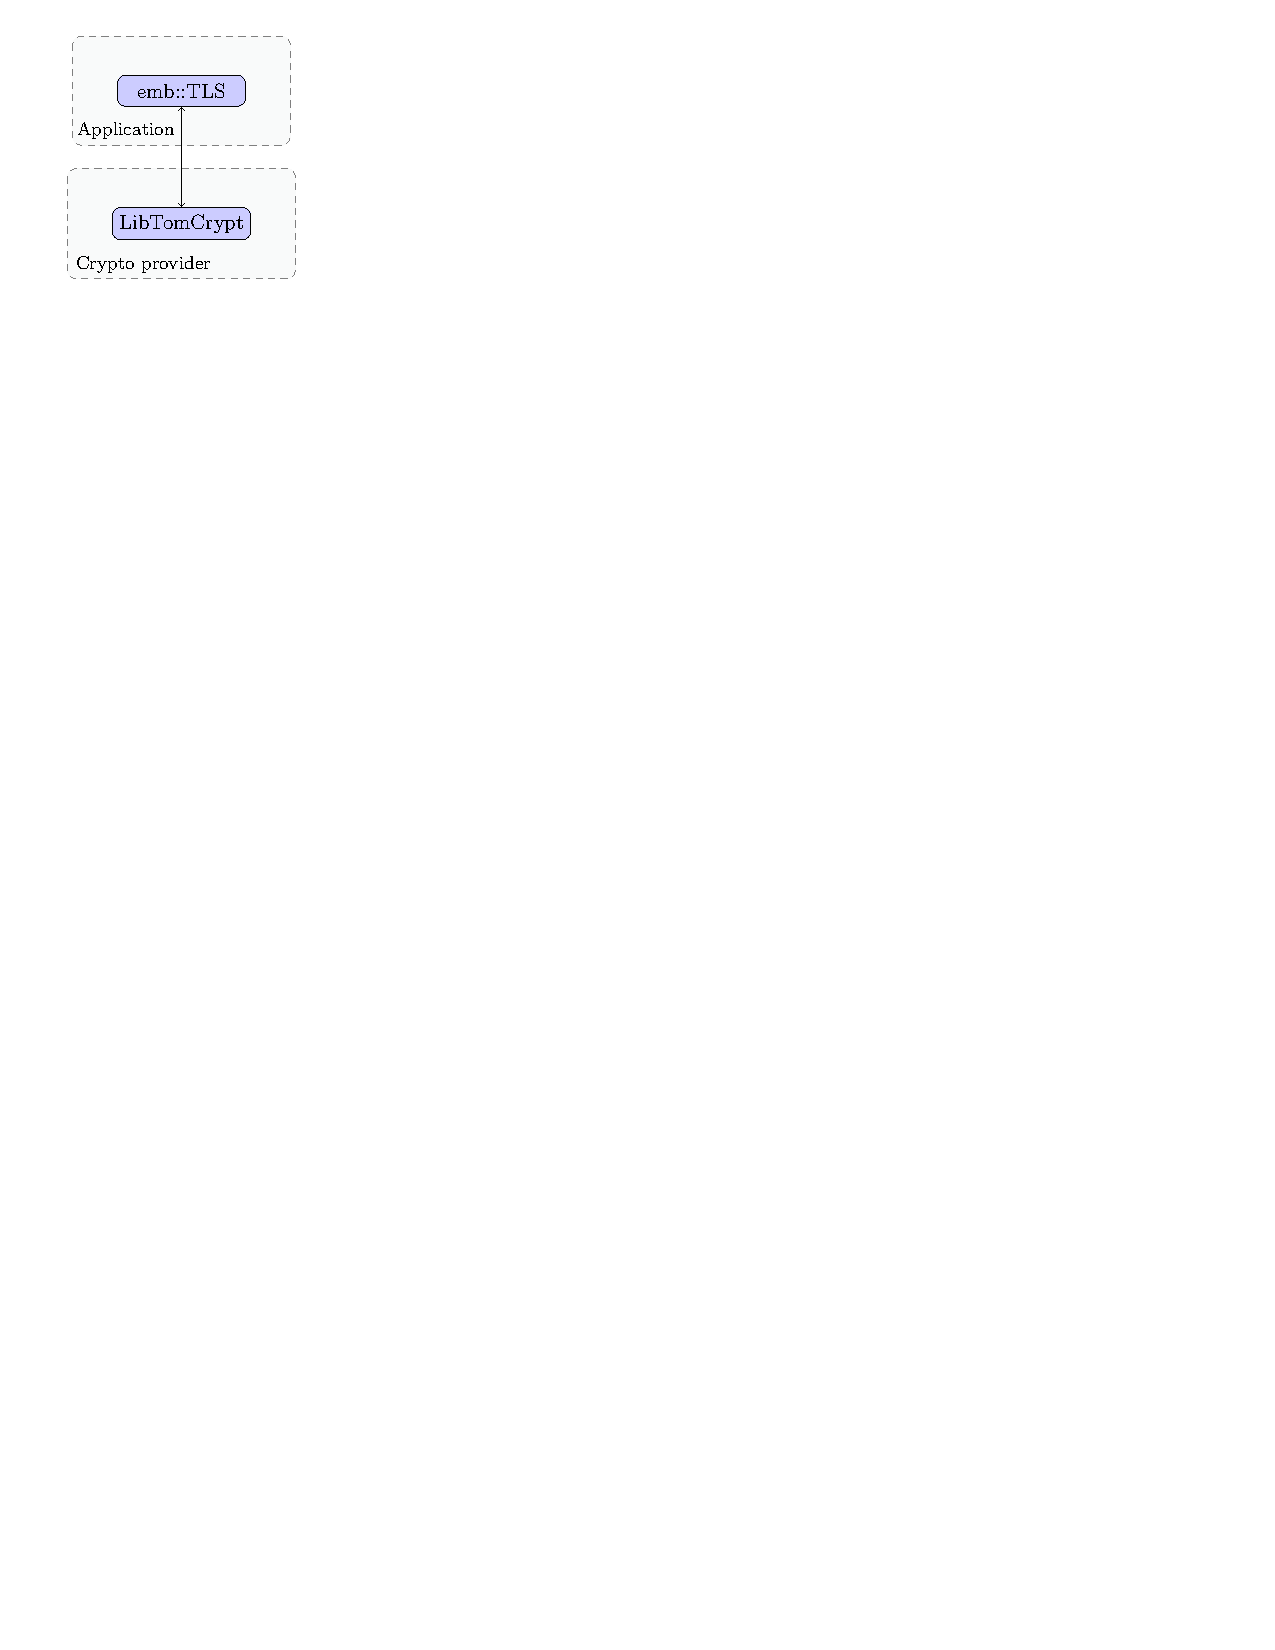
\includegraphics[trim=0cm 23.25cm 15cm 0cm,
height=6.5cm]{figures/intro_embtls.pdf}
\caption{\embtls's project}
\label{fig:motiv_embtls}
%}

\end{figure}
For this, a cryptographic provider (\tomcrypt) is used for the part of
cryptographic calculation needed for the application.
This cryptographic provider is an open-source cryptography software
library.
Problems with this implementation is that only \tomcrypt is
supported as cryptographic providers, meaning that no other libraries can be used
without changing the complete implementation for \embtls.

\begin{figure}[!ht]
\centering
%\frame{
% trim: left, bottom, right, up
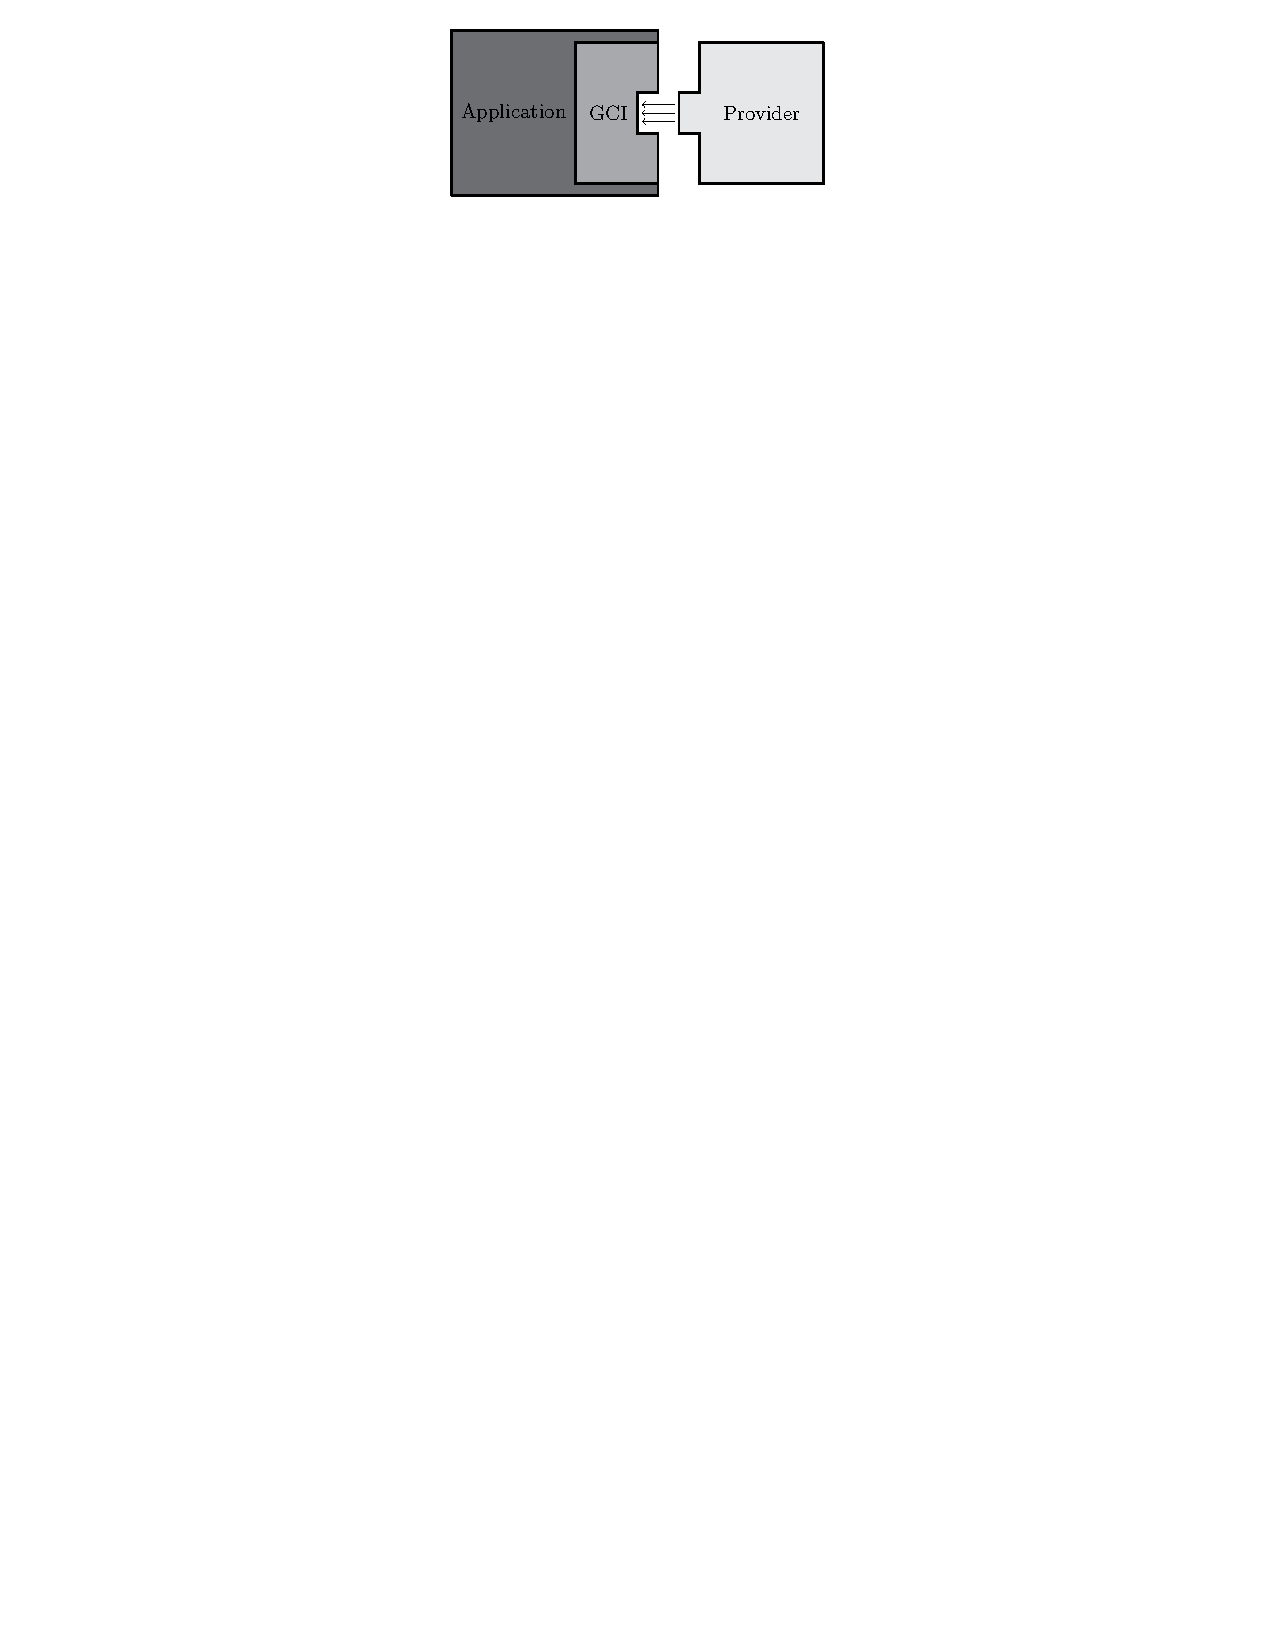
\includegraphics[trim=6cm 24.5cm 2cm 0cm, height=6cm]{figures/intro_gci.pdf}
\caption{Goal of the new implementation}
\label{fig:motiv_gci}
%}
\end{figure}
The goal of the project is therefore to create an interface, a Generic
Cryptographic Interface (GCI), to have a base of the existing cryptography
services and to have the possibility to easily change the providers only by
changing some lines in the interface, instead of the complete
implementation.\newline
Through to this new interface other new cryptographic algorithms may be
easier to add in the interface and to use for the application.\newline
As shown on the figure \ref{fig:motiv_gci}, the interface is implemented in the
application and nothing has to be changed.
The requirements for this Generic Cryptographic Interface (GCI) are listed
below:
\begin{enumerate}
  \item No hidden states shall be used in the interface, meaning that the
  behavior of the cryptographic algorithm functions should only be affected by
  the input parameters.
  All parameters written in input of the function will be used for the
  cryptographic algorithm and nothing else.
  \item Different cryptographic providers may be used for the cryptographic
  calculation. \newline
  That could be open-source cryptographic software libraries or hardware-based cryptographic modules.
  \item With the old version of the implementation (figure
  \ref{fig:motiv_embtls}), the application and the provider interact, meaning
  that when the provider needs informations from the application, this one just send them and
  vice-versa.
  With this new implementation (figure \ref{fig:motiv_gci}) the interface break
  this interaction. To always have this interaction, the interface shall receive
  the information from the application and the provider. These informations
  shall be easily used by both (application and provider) when needed.
\end{enumerate}
 
\chapter{Design}

%use of context
%work assymetric (do not need the end of a function to begin an other one)
%use of IDs 

\chapter{Initialisation of the interface}
	

\chapter{Context management}

%%%%%%%%%%%%%%%%%%%%%%%%%%%%%%%%%%%%%%%%%%%%%%%%%%%%%%%%%%%%
%					DEFINITION							   %
%%%%%%%%%%%%%%%%%%%%%%%%%%%%%%%%%%%%%%%%%%%%%%%%%%%%%%%%%%%%
\section{Definition}

The contexts represent the state of stateful algorithms. It allows to avoid the
hidden states in the interface, which mean that what is entering in the context
as configuration for an algorithm will be used for the calculation and no
parameters will be statically written in the functions of the interface.

%%%%%%%%%%%%%%%%%%%%%%%%%%%%%%%%%%%%%%%%%%%%%%%%%%%%%%%%%%%%
%					CREATE CONTEXT						   %
%%%%%%%%%%%%%%%%%%%%%%%%%%%%%%%%%%%%%%%%%%%%%%%%%%%%%%%%%%%%

\section{Create a context}
The princip of context is available for the following algorithms:
\begin{itemize}
  \item Hash
  \item Signature
  \item Symmetric cipher
  \item Asymmetric cipher
  \item Diffie-Hellman
\end{itemize}


\newpage

%%%%%%%%%%%%%%%%%%%%%%%%%%%%%%%%%%%%%%%%%%%%%%%%%%%%%%%%%%%%
%					HASH CONTEXT						   %
%%%%%%%%%%%%%%%%%%%%%%%%%%%%%%%%%%%%%%%%%%%%%%%%%%%%%%%%%%%%


\subsection{Hash context}
\label{hashCtx}

Prototype:

\begin{lstlisting}
/**
 * \fn							en_gciResult_t gciHashNewCtx( en_gciHashAlgo_t hashAlgo, GciCtxId_t* p_ctxID )
 * \brief						Create a new hash context and become an ID of it
 * \param [in]  hashAlgo 		Algorithm of the hash context
 * \param [out] p_ctxID			Pointer to the context's ID
 * @return						en_gciResult_Ok on success
 * @return						en_gciResult_Err on error
 */
en_gciResult_t gciHashNewCtx( en_gciHashAlgo_t hashAlgo, GciCtxId_t* p_ctxID );
\end{lstlisting}

The context is only needed to save the Hash algorithm.
For more informations of how to use a Hash context, see chapter \ref{hashfx}.

\newpage

%%%%%%%%%%%%%%%%%%%%%%%%%%%%%%%%%%%%%%%%%%%%%%%%%%%%%%%%%%%%
%					SIGN GEN CONTEXT					   %
%%%%%%%%%%%%%%%%%%%%%%%%%%%%%%%%%%%%%%%%%%%%%%%%%%%%%%%%%%%%

\subsection{Signature context (to generate a signature) }

Prototype:
\begin{lstlisting}

/**
 * \fn							en_gciResult_t gciSignGenNewCtx( const st_gciSignConfig_t* p_signConfig, GciKeyId_t keyID, GciCtxId_t* p_ctxID )
 * \brief						Create a new signature context and become an ID of it
 * \param [in]  p_signConfig	Pointer to the configuration of the signature
 * \param [in]  keyID			Key's ID
 * \param [out] p_ctxID			Pointer to the context's ID
 * @return						en_gciResult_Ok on success
 * @return						en_gciResult_Err on error
 */
en_gciResult_t gciSignGenNewCtx( const st_gciSignConfig_t* p_signConfig, GciKeyId_t keyID, GciCtxId_t* p_ctxID );

\end{lstlisting}

This context is used to save several different configuration to generate:
\begin{itemize}
  \item RSA signature
  \item DSA signature
  \item ECDSA signature
  \item Cipher Message Authentication Code (CMAC)
  \item Hash Message Authentication Code (HMAC)
\end{itemize}

Only one configuration is possible for one context. 
\newline
For more details about each configuration listed above see chapter
\ref{signature}

\newpage

%%%%%%%%%%%%%%%%%%%%%%%%%%%%%%%%%%%%%%%%%%%%%%%%%%%%%%%%%%%%
%					SIGN VFY CONTEXT					   %
%%%%%%%%%%%%%%%%%%%%%%%%%%%%%%%%%%%%%%%%%%%%%%%%%%%%%%%%%%%%

\subsection{Signature context (to verify a signature)}

Prototype:
\begin{lstlisting}

/**
 * \fn							en_gciResult_t gciSignVerifyNewCtx( const st_gciSignConfig_t* p_signConfig, GciKeyId_t keyID, GciCtxId_t* p_ctxID )
 * \brief						Create a new signature context and become an ID of it
 * \param [in]  p_signConfig	Pointer to the configuration of the signature
 * \param [in]  keyID			Key's ID
 * \param [out] p_ctxID			Pointer to the context's ID
 * @return						en_gciResult_Ok on success
 * @return						en_gciResult_Err on error
 */
en_gciResult_t gciSignVerifyNewCtx( const st_gciSignConfig_t* p_signConfig, GciKeyId_t keyID, GciCtxId_t* p_ctxID );

\end{lstlisting}

This context is used to save several different configuration to verify:
\begin{itemize}
  \item RSA signature
  \item DSA signature
  \item ECDSA signature
  \item Cipher Message Authentication Code (CMAC)
  \item Hash Message Authentication Code (HMAC)
\end{itemize}

Only one configuration is possible for one context. 
\newline
For more details about each configuration listed above see chapter
\ref{signature}

\newpage

%%%%%%%%%%%%%%%%%%%%%%%%%%%%%%%%%%%%%%%%%%%%%%%%%%%%%%%%%%%%
%					CIPHER CONTEXT						   %
%%%%%%%%%%%%%%%%%%%%%%%%%%%%%%%%%%%%%%%%%%%%%%%%%%%%%%%%%%%%

\subsection{Cipher context}

Prototype:
\begin{lstlisting}

/**
 * \fn							en_gciResult_t gciCipherNewCtx( const st_gciCipherConfig_t* p_ciphConfig, GciKeyId_t keyID, GciCtxId_t* p_ctxID )
 * \brief						Create a new symmetric cipher context
 * \param [in]	p_ciphConfig	Pointer to the configuration of the symmetric cipher
 * \param [in]  keyID			Key's ID
 * \param [out] p_ctxID			Pointer to the context's ID
 * @return						en_gciResult_Ok on success
 * @return						en_gciResult_Err on error
 */
en_gciResult_t gciCipherNewCtx( const st_gciCipherConfig_t* p_ciphConfig, GciKeyId_t keyID, GciCtxId_t* p_ctxID );

\end{lstlisting}

This context is use to encrypt a plaintext or decrypt a ciphertext.

The cipher algorithm which could be used are:
\begin{itemize}
  \item Symmetric stream cipher RC4
  \item Symmetric block cipher AES
  \item Symmetric block cipher DES
  \item Symmetric block cipher 3DES
  \item Asymmetric cipher RSA
\end{itemize}

For more details of each configuration see chapter \ref{cipher}

\newpage

%%%%%%%%%%%%%%%%%%%%%%%%%%%%%%%%%%%%%%%%%%%%%%%%%%%%%%%%%%%%
%					DH CONTEXT							   %
%%%%%%%%%%%%%%%%%%%%%%%%%%%%%%%%%%%%%%%%%%%%%%%%%%%%%%%%%%%%

\subsection{Diffie-Hellmann context}

Prototype:
\begin{lstlisting}

/**
 * \fn							en_gciResult_t gciDhNewCtx( const st_gciDhConfig_t* p_dhConfig, GciCtxId_t* p_ctxID )
 * \brief						Create a new Diffie-Hellman context
 * \param [in]  p_dhConfig		Pointer to the configuration of the Diffie-Hellman
 * \param [out] p_ctxID			Pointer to the context's ID
 * @return						en_gciResult_Ok on success
 * @return						en_gciResult_Err on error
 */
en_gciResult_t gciDhNewCtx( const st_gciDhConfig_t* p_dhConfig, GciCtxId_t* p_ctxID );

\end{lstlisting}

This context is used to created :
\begin{itemize}
  \item Diffie-Hellman
  \item Elliptic Curve Diffie-Hellman
  \item Shared secret for Diffie-Hellman
  \item Shared secret for Elliptic Curve
Diffie-Hellman
\end{itemize}

Furthermore, the private key generated must be saved internally. 

For more information about the configuration and the generation of the
Diffie-Hellman/Elliptic Curve Diffie-Hellman key pair see chapter \ref{dhKeys}

For more informations about the generation of the shared secret see
chapter \ref{dhSec}

\newpage

%%%%%%%%%%%%%%%%%%%%%%%%%%%%%%%%%%%%%%%%%%%%%%%%%%%%%%%%%%%%
%					CLONE CONTEXT						   %
%%%%%%%%%%%%%%%%%%%%%%%%%%%%%%%%%%%%%%%%%%%%%%%%%%%%%%%%%%%%

\section{Clone an existing context}

One of the inconvenient of the interface comes from the finish part, where the
last calculation is done.
For the hash algorithm and the signature algorithm, when the digest/signature is
calculated, no more updates could be done with the last configuration and
with the previous updates.

The solution of this problem is the clone of the context.

When the digest/signature has to be calculated but the configuration and the
previous updates should be kept, the clone of the hash/signature context allows
to copy the configuration and the previous updates. Two contexts are identical
but one is use for the calculation of the digest/signature and the other one for
futur updates.

\subsection{Hash context}
Prototype:
\begin{lstlisting}

/*!
 * \fn 							en_gciResult_t gciHashCtxClone( GciCtxId_t idSrc, GciCtxId_t* p_idDest )
 * \brief						Clone a context
 * \param [in]  idSrc			The context which will be cloned
 * \param [out] p_idDest		Pointer to the context ID where the source context is cloned
 * @return						en_gciResult_Ok on success
 * @return						en_gciResult_Err on error
 */
en_gciResult_t gciHashCtxClone( GciCtxId_t idSrc, GciCtxId_t* p_idDest );

\end{lstlisting}

\subsection{Both Signature context}
Prototype:
\begin{lstlisting}

/*!
 * \fn 							en_gciResult_t gciSignCtxClone( GciCtxId_t idSrc, GciCtxId_t* p_idDest )
 * \brief						Clone a context
 * \param [in]  idSrc			The context which will be cloned
 * \param [out] p_idDest		Pointer to the context ID where the source context is cloned
 * @return						en_gciResult_Ok on success
 * @return						en_gciResult_Err on error
 */
en_gciResult_t gciSignCtxClone( GciCtxId_t idSrc, GciCtxId_t* p_idDest );

\end{lstlisting}

\newpage

%%%%%%%%%%%%%%%%%%%%%%%%%%%%%%%%%%%%%%%%%%%%%%%%%%%%%%%%%%%%
%					DELETE CONTEXT						   %
%%%%%%%%%%%%%%%%%%%%%%%%%%%%%%%%%%%%%%%%%%%%%%%%%%%%%%%%%%%%
\section{Delete an existing context}
\label{delCtx}

When the context is not needed anymore, it can be removed and be used for an
other configuration, which can be completely different as the previous one.

Prototype:
\begin{lstlisting}

/*!
 * \fn 							en_gciResult_t gciCtxRelease( GciCtxId_t ctxID )
 * \brief						Release a context
 * \param [in] ctxID			Context's ID
 * @return						en_gciResult_Ok on success
 * @return						en_gciResult_Err on error
 */
en_gciResult_t gciCtxRelease( GciCtxId_t ctxID );

\end{lstlisting}

\include{chapter/information}
\chapter{Hash functions}
\label{hashfx}

\section{Algorithm of hash}

\begin{lstlisting}

/**
 * \enum 					en_GciHashAlgo
 * \brief					Enumeration for Hash algorithms
 */
typedef enum en_GciHashAlgo
{
	/** Invalid Hash */
	en_gciHashAlgo_Invalid,
	/** MD5 Hash */
	en_gciHashAlgo_MD5,
	/** SHA1 Hash */
	en_gciHashAlgo_SHA1,
	/** SHA224 Hash */
	en_gciHashAlgo_SHA224,
	/** SHA256 Hash */
	en_gciHashAlgo_SHA256,
	/** SHA384 Hash */
	en_gciHashAlgo_SHA384,
	/** SHA512 Hash */
	en_gciHashAlgo_SHA512,
	/** No hash algorithm used */
	en_gciHashAlgo_None=0xFF
} en_gciHashAlgo_t;

\end{lstlisting}


\section{Prototypes}

Create a new Hash context:
\begin{lstlisting}

/**
 * \fn							en_gciResult_t gciHashNewCtx( en_gciHashAlgo_t hashAlgo, GciCtxId_t* p_ctxID )
 * \brief						Create a new hash context and become an ID of it
 * \param [in]  hashAlgo 		Algorithm of the hash context
 * \param [out] p_ctxID			Pointer to the context's ID
 * @return						en_gciResult_Ok on success
 * @return						en_gciResult_Err on error
 */
en_gciResult_t gciHashNewCtx( en_gciHashAlgo_t hashAlgo, GciCtxId_t* p_ctxID );

\end{lstlisting}

Update the Hash context with data:
\begin{lstlisting}

/**
 * \fn							en_gciResult_t gciHashUpdate( GciCtxId_t ctxID, const uint8_t* p_blockMsg, size_t blockLen )
 * \brief						Add block of the message
 * \param [in]  ctxID	 		Context's ID
 * \param [in]  p_blockMsg		Pointer to the block of the message
 * \param [in]  blockLen		Block message's length
 * @return						en_gciResult_Ok on success
 * @return						en_gciResult_Err on error
 */
en_gciResult_t gciHashUpdate( GciCtxId_t ctxID, const uint8_t* p_blockMsg, size_t blockLen );

\end{lstlisting}

Clone the context:
\begin{lstlisting}

/*!
 * \fn 							en_gciResult_t gciHashCtxClone( GciCtxId_t idSrc, GciCtxId_t* p_idDest )
 * \brief						Clone a context
 * \param [in]  idSrc			The context which will be cloned
 * \param [out] p_idDest		Pointer to the context ID where the source context is cloned
 * @return						en_gciResult_Ok on success
 * @return						en_gciResult_Err on error
 */
en_gciResult_t gciHashCtxClone( GciCtxId_t idSrc, GciCtxId_t* p_idDest );

\end{lstlisting}


Get the digest of the Hash:
\begin{lstlisting}

/**
 * \fn							en_gciResult_t gciHashFinish( GciCtxId_t ctxID, uint8_t* p_digest, size_t* p_digestLen )
 * \brief						Get the digest of the message after adding all the block of the message
 * \param [in]  ctxID	 		Context's ID
 * \param [out] p_digest		Pointer to the digest of the complete message added
 * \param [out] p_digestLen		Pointer to the length of the digest in bytes
 * @return						en_gciResult_Ok on success
 * @return						en_gciResult_Err on error
 */
en_gciResult_t gciHashFinish( GciCtxId_t ctxID, uint8_t* p_digest, size_t* p_digestLen );

\end{lstlisting}

\newpage

\section{Steps to hash (Example)}

\begin{lstlisting}
#include <stdio.h>
#include <stdlib.h>
#include <string.h>
#include "crypto_iface.h"

int main(int argc , char *argv[])
{
    /* Error Management */
    en_gciResult_t err;

    /* MD5 context ID */
    GciCtxId_t md5CtxID, md5CloneCtxID;

    /* Messages to hash */
    uint8_t a_data1[10] = {"Hello!"};
    uint8_t a_data2[30] = {"This is a Hash MD5 test"};
    uint8_t a_data3[10] = {"Thank you."};

    size_t data1Len = strlen(a_data1);
    size_t data2Len = strlen(a_data2);
    size_t data3Len = strlen(a_data3);

    int i;

    /* a MD5 digest is always 128 bits -> 16 bytes */
    uint8_t a_digest[GCI_MD5_SIZE_BYTES];

    /* Initialize the buffer */
    memset(a_digest, 0, GCI_MD5_SIZE_BYTES);

    size_t digestLen = 0;

    /* Create a new hash MD5 context */
    err = gciHashNewCtx(en_gciHashAlgo_MD5, &md5CtxID);

    /* Error coming from the creation of a new MD5-Hash context */
    if(err != en_gciResult_Ok)
    {
        printf("GCI Error in gciHashNewCtx: MD5");
    }

    /* Add the first data by updating the hash context */
    err = gciHashUpdate(md5CtxID, a_data1, data1Len);

    /* Error coming from the updating of the hash context with data1 */
    if(err != en_gciResult_Ok)
    {
        printf("GCI Error in gciHashUpdate: MD5");
    }

    /* Add the second data by updating the hash context */
    err = gciHashUpdate(md5CtxID, a_data2, data2Len);

    /* Error coming from the updating of the hash context with data2 */
    if(err != en_gciResult_Ok)
    {
        printf("GCI Error in gciHashUpdate: MD5");
    }

    /* Clone the context */
    err = gciHashCtxClone(md5CtxID, &md5CloneCtxID);
    if(err != en_gciResult_Ok)
    {
        printf("GCI Error in gciHashCtxClone: MD5");
    }

    /* Get the digest of this message */
    err = gciHashFinish(md5CtxID, a_digest, &digestLen);
    if(err != en_gciResult_Ok)
    {
        printf("GCI Error in gciHashFinish: MD5");
    }

    else
    {
        printf("GCI Info: Digest1 = ");
        for(i = 0; i < GCI_MD5_SIZE_BYTES; i++)
        {
            printf("%d", a_digest[i]);
        }
    }

    /* Initialize the buffer */
    memset(a_digest, 0, GCI_MD5_SIZE_BYTES);

    /* Add the third data by updating the hash context */
    err = gciHashUpdate(md5CloneCtxID, a_data3, data3Len);

    /* Error coming from the updating of the hash context with data3 */
    if(err != en_gciResult_Ok)
    {
        printf("GCI Error in gciHashUpdate: MD5");
    }

    /* Get the digest of this message */
    err = gciHashFinish(md5CloneCtxID, a_digest, &digestLen);
    if(err != en_gciResult_Ok)
    {
        printf("GCI Error in gciHashFinish: MD5");
    }

    else
    {
        printf("\r\nGCI Info: Digest2 = ");
        for(i=0; i<GCI_MD5_SIZE_BYTES; i++)
        {
            printf("%d", a_digest[i]);
        }

    }

    printf("\r\n");

    /* Delete the contexts */
    gciCtxRelease(md5CtxID);
    gciCtxRelease(md5CloneCtxID);

}

\end{lstlisting}
\chapter{Signature/MAC algorithms}
\label{sign}

\section{Configuration of Signature / MAC algorithms}

\begin{center}

\begin{tabular}{| c | c|}
 \hline
Algorithm				& Parameter \\
\Gline
RSA						& en\_gciSignAlgo\_RSA \\
\hline
DSA						& en\_gciSignAlgo\_DSA \\
\hline
ECDSA					& en\_gciSignAlgo\_ECDSA \\
\hline
MAC ISO9797 Algorithm 1	& en\_gciSignAlgo\_MAC\_ISO9797\_ALG1 \\
\hline
MAC ISO9797 Algorithm 3 & en\_gciSignAlgo\_MAC\_ISO9797\_ALG3 \\
\hline
Cipher-based MAC		& en\_gciSignAlgo\_CMAC \\
\hline
Hash-based MAC			& en\_gciSignAlgo\_HMAC \\
\hline
\end{tabular}
\captionof{table}{Signature/MAC algorithms (en\_gciSignAlgo\_t) }
\label{tab:sign_algo}

\end{center}



\begin{center}

\begin{tabular}{| c | c | c |}
\hline
Parameter		& Type \\				
\Gline
algo			& en\_gciSignAlgo\_t \\
\hline
hash			& en\_gciHashAlgo\_t \\
\hline
signConfigRsa	& st\_gciSignRsaConfig\_t \\	
(If RSA is used as algorithm)	& \\
\hline
signConfigCmac	& st\_gciSignCmacConfig\_t \\
(If CMAC is used as algorithm)	& \\
\hline	


\end{tabular}
\captionof{table}{Configuration of Signature/MAC algorithms
(st\_gciSignConfig\_t))}
\label{tab:sign_conf}

\end{center}



\section{Prototypes}
Two differents use of the signature are available.\newline
The first one is the generation of a signature, which will sign the datas
updated (see
section \ref{signGen} for more details.

The second one is the verification of a signature, which will sign the datas
updated but will at the end compared with this entered in the function (see
section \ref{signVfy} for more details).

\subsection{Creation of a context}

There is two possibilities of use for the signature context. The first one is to
generate a signature and the second one to verify a signature. It has been split
because some known provider needs to do the difference between the twice
possibilities.

\begin{lstlisting}
en_gciResult_t gciSignGenNewCtx( const st_gciSignConfig_t* p_signConfig,
GciKeyId_t keyID, GciCtxId_t* p_ctxID )
\end{lstlisting}

\begin{lstlisting}
en_gciResult_t gciSignVerifyNewCtx( const st_gciSignConfig_t* p_signConfig,
GciKeyId_t keyID, GciCtxId_t* p_ctxID )
\end{lstlisting}


\begin{center}

\begin{tabular}{| c | *{3}{c|}}
 \hline
 Direction 	& Type 						& Parameter 			& Definition \\
 \Gline
 Input 	   	& st\_gciSignConfig\_t*	 	& p\_signConfig			& Pointer to the
 configuration of the signature
 \\
 \hline
 Input	   	& GciKeyId\_t			 	& keyID					& ID of the key uses to sign \\
 \hline
Output		& GciCtxId\_t* 				& p\_ctxID				& Pointer to the
context's ID \\
\hline
\end{tabular}
\captionof{table}{Parameters for the creation of a signature/MAC context}
\label{tab:sign_ctx}

\end{center}

\subsubsection*{RSA}

The hash algorithm can be used if the
updated data has to be hashed before to be signed. If not, this parameter should be
configure as en\_gciHashAlgo\_None.

\begin{center}

\begin{tabular}{| c | *{2}{c|}}
 \hline
 Parameter 		& Configuration			& Prohibition(s) \\
 \Gline
 algo 	   		& en\_gciSignAlgo\_Rsa 	& - \\
\hline
 hash			& en\_gciHashAlgo\_t  	& en\_gciHash\_Invalid \\					
 \hline
 padding		& en\_gciPadding\_t 	& en\_gciPadding\_Invalid \\
 				&						& en\_gciPadding\_None \\
 \hline
\end{tabular}
\captionof{table}{Configuration of RSA Signature Scheme Algorithms
(st\_gciSignConfig\_t)}
\label{tab:sign_rsa}

\end{center}

\subsubsection*{DSA}

\begin{center}

\begin{tabular}{| c | *{2}{c|}}
 \hline
 Parameter 		& Configuration			& Prohibition(s) \\
 \Gline
 algo 	   		& en\_gciSignAlgo\_Dsa 	& - \\
\hline
 hash			& en\_gciHashAlgo\_t  	& en\_gciHash\_Invalid \\					
 \hline
\end{tabular}
\captionof{table}{Configuration of Digital Signature Algorithms
(st\_gciSignConfig\_t)}
\label{tab:sign_dsa}

\end{center}

\subsubsection*{ECDSA}

\begin{center}

\begin{tabular}{| c | *{2}{c|}}
 \hline
 Parameter 		& Configuration				& Prohibition(s) \\
 \Gline
 algo 	   		& en\_gciSignAlgo\_Ecdsa 	& - \\
\hline
 hash			& en\_gciHashAlgo\_t  		& en\_gciHash\_Invalid \\					
 \hline
\end{tabular}
\captionof{table}{Configuration of Elliptic Curve Digital Signature Algorithms
(st\_gciSignConfig\_t)}
\label{tab:sign_ecdsa}

\end{center}

\subsubsection*{Cipher-based MAC (CMAC)}

\begin{center}

\begin{tabular}{| c | *{2}{c|}}
 \hline
 Parameter 		& Configuration				& Prohibition(s) \\
 \Gline
 algo 	   		& en\_gciSignAlgo\_Cmac 	& - \\
\hline
 hash			& en\_gciHashAlgo\_t  		& en\_gciHash\_Invalid \\					
 \hline
 block			& en\_gciBlockMode\_t		& en\_gciBlockMode\_Invalid \\
 				&							& en\_gciBlockMode\_None \\
 \hline
 padding		& en\_gciPadding\_t			& en\_gciPadding\_Invalid \\
 \hline
 iv.data		& uint8\_t*					& NULL \\ 
 iv.len			& size\_t					& value less or equal than 0 \\	
 \hline
\end{tabular}
\captionof{table}{Configuration of Cipher-based MAC
(st\_gciSignConfig\_t)}
\label{tab:sign_cmac}

\end{center}

\subsubsection*{Hash-based MAC (HMAC)}

\begin{center}

\begin{tabular}{| c | *{2}{c|}}
 \hline
 Parameter 		& Configuration				& Prohibition(s) \\
 \Gline
 algo 	   		& en\_gciSignAlgo\_Hmac 	& - \\
\hline
 hash			& en\_gciHashAlgo\_t  		& en\_gciHash\_Invalid \\	
 				&							& en\_gciHash\_None \\				
 \hline
\end{tabular}
\captionof{table}{Configuration of Hash-based MAC
(st\_gciSignConfig\_t)}
\label{tab:sign_hmac}

\end{center}

\subsection{Update of the context}

The update of the context for generating and verificate a signature is the same.
The data have to be added to get a signature.

\begin{lstlisting}
en_gciResult_t gciSignUpdate( GciCtxId_t ctxID, const uint8_t* p_blockMsg,
size_t blockLen )
\end{lstlisting}

\begin{center}

\begin{tabular}{| c | *{3}{c|}}
 \hline
 Direction 	& Type 				& Parameter 			& Definition \\
 \Gline
 Input 	   	& GciCtxId\_t		& ctxID					& Context's ID \\
 \hline
 Input	   	& uint8\_t*			& p\_blockMsg			& Pointer to the message to sign \\
 \hline
 Input		& size\_t			& blockLen				& Length of message \\
 \hline
\end{tabular}
\captionof{table}{Parameters for the update of a signature/MAC context}
\label{tab:sign_upd}

\end{center}

\subsection{Clone of signature/MAC algorithm}

\begin{lstlisting}
en_gciResult_t gciSignCtxClone( GciCtxId_t idSrc, GciCtxId_t* p_idDest )
\end{lstlisting}


\begin{center}

\begin{tabular}{| c | *{3}{c|}}
 \hline
 Direction 	& Type 						& Parameter 			& Definition \\
 \Gline
 Input 	   	& GciCtxId\_t			 	& idSrc					& The context which will be cloned \\
 \hline
Output		& GciCtxId\_t*	 			& p\_idDest				& Pointer to the clone context ID \\
\hline
 
\end{tabular}
\captionof{table}{Parameters for the clone of a signature/MAC context}
\label{tab:sign_clone}

\end{center}

\subsection{Calculation / Verification of the signature}
After the data have been added to the context, if the context is to generate a
signature, than the signature will be compted and returned.
If the context if to verify a signature, than the signature to verify has to be
added to the function. Internally the signature with the updated data will be
computed but ot returned. Only if the the returning value of the function
indicates if the signatures are the same or not.

\begin{lstlisting}
en_gciResult_t gciSignGenFinish( GciCtxId_t ctxID, uint8_t* p_sign, size_t*
p_signLen )
\end{lstlisting}

\begin{center}

\begin{tabular}{| c | *{3}{c|}}
 \hline
 Direction 	& Type 				& Parameter 			& Definition \\
 \Gline
 Input 	   	& GciCtxId\_t		& ctxID					& Context's ID \\
 \hline
 Input	   	& uint8\_t*			& p\_sign				& Pointer to the generated signature \\
 \hline
 Input		& size\_t*			& signLen				& Pointer to the length of the generated
 signature \\
 \hline
\end{tabular}
\captionof{table}{Parameters for the computation of a signature/MAC}
\label{tab:sign_gen_fin}

\end{center}

\begin{lstlisting}
en_gciResult_t gciSignVerifyFinish( GciCtxId_t ctxID, const uint8_t* p_sign,
size_t signLen )
\end{lstlisting}

\begin{center}

\begin{tabular}{| c | *{3}{c|}}
 \hline
 Direction 	& Type 				& Parameter 			& Definition \\
 \Gline
 Input 	   	& GciCtxId\_t		& ctxID					& Context's ID \\
 \hline
 Input	   	& uint8\_t*			& p\_sign				& Pointer to the signature to verify \\
 \hline
 Input		& size\_t			& signLen				& Length of the signature to verify\\
 \hline
\end{tabular}
\captionof{table}{Parameters for the verification of a signature/MAC}
\label{tab:sign_vfy_fin}

\end{center}

\section{Step to generate a signature}
For this example the keys have already been added previously to the interface 
and an ID returned.
\begin{lstlisting}

	#include <stdio.h>
	#include <stdlib.h>
	#include <string.h>
	#include "crypto_iface.h"

	int main(int argc , char *argv[])
	{

	    /* Configuration of a RSA signature */
	    st_gciSignConfig_t signConfig = {.algo = en_gciSignAlgo_Rsa,
	        .hash = en_gciHashAlgo_None
	    };

	    signConfig.un_signConfig.signConfigRsa.padding = en_gciPadding_Pkcs1_Emsa;


	    /* Error Management */
	    en_gciResult_t err;

	    /* Messages to hash */
	    uint8_t a_data1[10] = {"Hello!"};
	    uint8_t a_data2[30] = {"This is a RSA Signature test"};
	    uint8_t a_data3[10] = {"Thank you."};

	    size_t data1Len = strlen(a_data1);
	    size_t data2Len = strlen(a_data2);
	    size_t data3Len = strlen(a_data3);

	    /* Buffer for the signature */
	    uint8_t a_signature[30];
	    size_t signLen;


	    int i;

	    /* RSA context ID */
	    GciCtxId_t rsaCtxID;

	    /* Init of the signature */
	    memset(a_signature, 0, 30);
	    signLen = 0;

	    /* Creation of the signature context with the RSA private key */
	    err = gciSignGenNewCtx(&signConfig, rsaPrivKeyID, &rsaCtxID);

	    /* Error coming from the creation of a new MD5-Hash context */
	    if(err != en_gciResult_Ok)
	    {
	        printf("GCI Error in gciSignGenNewCtx: RSA");
	    }

	    /* First update of the signature */
	    err = gciSignUpdate(rsaCtxID, a_data1, data1Len);

	    /* Error coming from the update of a RSA-signature context */
	    if(err != en_gciResult_Ok)
	    {
	        printf("GCI Error in gciSignUpdate: RSA");
	    }

	    /* Second update of the signature */
	    err = gciSignUpdate(rsaCtxID, a_data2, data2Len);

	    /* Error coming from the update of a RSA-signature context */
	    if(err != en_gciResult_Ok)
	    {
	        printf("GCI Error in gciSignUpdate: RSA");
	    }

	    /* Third update of the signature */
	    err = gciSignUpdate(rsaCtxID, a_data3, data3Len);

	    /* Error coming from the update of a RSA-signature context */
	    if(err != en_gciResult_Ok)
	    {
	        printf("GCI Error in gciSignUpdate: RSA");
	    }

	    /* Generation of the signature */
	    err = gciSignGenFinish(rsaCtxID, a_signature, &signLen);

	    /* Error coming from the generation of a RSA-signature */
	    if(err != en_gciResult_Ok)
	    {
	        printf("GCI Error in gciSignGenFinish: RSA");
	    }

	    else
	    {
	        printf("GCI Info: Signature = ");
	        for(i = 0; i < signLen; i++)
	        {
	            printf("%d", a_signature[i]);
	        }
	    }

	    /* Delete the context */
	    gciCtxRelease(rsaCtxID);

	}
\end{lstlisting}

\chapter{Generation of key pair}

\section{Configuration of a key pair}
\subsection{RSA}
\subsection{Digital Signature Algorithm (DSA)}
\subsection{Elliptic Curve Digital Signature Algorithm (ECDSA)}

\section{Steps to generate a key pair}
\chapter{Cipher algorithms}

\section{Configuration of a symmetric cipher}

\section{Configuration of an asymmetric cipher}

\section{Encrypt a plaintext}

\section{Decrypt a ciphertext}
\chapter{Generate Diffie-Hellmann key pair}

\section{Configuration of a Diffie-Hellmann key pair}
\subsection{Diffie-Hellmann (DH)}
\subsection{Elliptic Curve Diffie Hellmann (ECDH)}


\section{Steps to generate a Diffie-Hellmann key pair}
\chapter{Calculation of a Diffie-Hellmann shared secret}
\label{dhSec}

\section{Steps to calculate a shared secret}
\chapter{Pseudo-Random Number Generator}

\section{Generate a pseudo-random number}

\section{Seed a pseudo-random number}
\chapter{Key management}
\label{keyManag}

The hardware-based cryptographic modules use a key management. This institute
wants to use this key management, that's why the interface shall have a key
management too.

\section{Save a key and get an ID}

There is two possibilities about the value of the given ID. Either the ID is
previously initialized to -1, so will the smallest value free for an ID
returned, or the ID can be initialized to a value greater or equal to 0 to be
the same as a context ID for example, so if this value is free, the key will be
saved at this specified ID.

\begin{lstlisting}
en_gciResult_t gciKeyPut( const st_gciKey_t* p_key, GciKeyId_t* p_keyID )
\end{lstlisting}

\begin{center}

\begin{tabular}{| c | *{3}{c|}}
 \hline
 Direction 	& Type 				& Parameter 			& Definition \\
 \Gline
 Input 	   	& st\_gciKey\_t*	& p\_key				& Pointer to the key to save \\
 \hline
 Output	   	& GciKeyId\_t*		& p\_keyID				& Pointer to the ID of the saved key \\
 \hline
\end{tabular}
\captionof{table}{Parameters for to put a key}
\label{tab:key_put}

\end{center}

\section{Get of a saved key with its ID}

\begin{lstlisting}
en_gciResult_t gciKeyGet( GciKeyId_t keyID, st_gciKey_t* p_key )
\end{lstlisting}

\begin{center}

\begin{tabular}{| c | *{3}{c|}}
 \hline
 Direction 	& Type 				& Parameter 			& Definition \\
 \Gline
 Input 	   	& GciKeyId\_t		& p\_key				& ID of the key to get \\
 \hline
 Output	   	& st\_gciKey\_t*	& p\_keyID				& Pointer to the saved key \\
 \hline
\end{tabular}
\captionof{table}{Parameters for to get a key}
\label{tab:key_get}

\end{center}

\section{Delete a key}

\begin{lstlisting}
en_gciResult_t gciKeyDelete( GciKeyId_t keyID  )
\end{lstlisting}

\begin{center}

\begin{tabular}{| c | *{3}{c|}}
 \hline
 Direction 	& Type 				& Parameter 			& Definition \\
 \Gline
 Input 	   	& GciKeyId\_t		& p\_key				& ID of the key to delete \\
 \hline
\end{tabular}
\captionof{table}{Parameters for to delete a key}
\label{tab:key_del}

\end{center}




%----------------------------------------------------------------------------------------
%	Bibliography
%----------------------------------------------------------------------------------------

%% prints every entry of the bib file -- useful in a state where is no cite
%\appendix
\nocite{*}
%\printbibliography
\bibliographystyle{plain}
\bibliography{bib/bibliography}


%----------------------------------------------------------------------------------------
%	Appendix
%----------------------------------------------------------------------------------------
%% add possible appendix 
%%\appendix
%%\addpart*{Appendix}
%%\addcontentsline{toc}{chapter}{Appendix}

\begin{appendices}
\chapter{Other parameters}

\section{Global types}

%----------------------------------------------------------------------------------------
%	Context ID
%----------------------------------------------------------------------------------------

\begin{center}

\begin{tabular}{| c | c | c |}
 \hline
Name			& Type			& Definition \\
\Gline
GciCtxId\_t		& int 			& Context's ID \\
\hline
\end{tabular}
\captionof{table}{Context's ID (st\_gciCtxId\_t) }
\label{tab:app_ctx}

\end{center}

%----------------------------------------------------------------------------------------
%	Key ID
%----------------------------------------------------------------------------------------

\begin{center}

\begin{tabular}{| c | c | c |}
 \hline
Name			& Type			& Definition \\
\Gline
GciKeyId\_t		& int 			& Key's ID \\
\hline
\end{tabular}
\captionof{table}{Key's ID (st\_gciKeyId\_t) }
\label{tab:app_key}

\end{center}

%----------------------------------------------------------------------------------------
%	Big Int
%----------------------------------------------------------------------------------------

\begin{center}

\begin{tabular}{| c | c | c |}
 \hline
Name		& Type			& Definition \\
\Gline
len			& size\_t 		& Length of the big number (in bytes) \\
\hline
data		& uint8\_t*		& Big numbre (data) \\
\hline
\end{tabular}
\captionof{table}{Parameters of a big number (st\_gciBigInt\_t) }
\label{tab:app_bn}

\end{center}

%----------------------------------------------------------------------------------------
%	Buffer
%----------------------------------------------------------------------------------------

\begin{center}

\begin{tabular}{| c | c | c |}
 \hline
Name		& Type			& Definition \\
\Gline
len			& size\_t 		& Length of the buffer (in bytes) \\
\hline
data		& uint8\_t*		& Buffer (data) \\
\hline
\end{tabular}
\captionof{table}{Parameters of a buffer (st\_gciBuffer\_t) }
\label{tab:app_buf}

\end{center}


\section{Managements}

%----------------------------------------------------------------------------------------
%	Result
%----------------------------------------------------------------------------------------

\begin{center}

\begin{tabular}{| c | c|}
 \hline
Name					& Parameter \\
\Gline
No errors				& en\_gciResult\_Ok \\
\hline
Error(s)				& en\_gciResult\_Err \\
\hline
\end{tabular}
\captionof{table}{Error management (en\_gciResult\_t) }
\label{tab:app_res}

\end{center}


%----------------------------------------------------------------------------------------
%	Info
%----------------------------------------------------------------------------------------

\begin{center}

\begin{tabular}{| c | c|}
 \hline
Name							& Parameter \\
\Gline
Invalid Information				& en\_gciInfo\_Invalid \\
\hline
Name of the available curves	& en\_gciInfo\_CurveName \\
\hline
\end{tabular}
\captionof{table}{Information management (en\_gciInfo\_t) }
\label{tab:app_info}

\end{center}



\section{Block modes}

%----------------------------------------------------------------------------------------
%	Block mode
%----------------------------------------------------------------------------------------

\begin{center}

\begin{tabular}{| c | c|}
 \hline
Name					& Parameter \\
\Gline
Invalid Block mode		& en\_gciBlockMode\_Invalid \\
\hline
CBC						& en\_gciBlockMode\_Cbc \\
\hline
ECB						& en\_gciBlockMode\_Ecb \\
\hline
CFB						& en\_gciBlockMode\_Cfb \\
\hline
OFB						& en\_gciBlockMode\_Ofb \\
\hline
GCM						& en\_gciBlockMode\_Gcm \\
\hline
No block mode			& en\_gciBlockMode\_None \\
\hline
\end{tabular}
\captionof{table}{Block modes (en\_gciBlockMode\_t) }
\label{tab:app_bm}

\end{center}

\section{Paddings}

%----------------------------------------------------------------------------------------
%	Padding
%----------------------------------------------------------------------------------------

\begin{center}

\begin{tabular}{| c | c|}
 \hline
Name					& Parameter \\
\Gline
Invalid Padding			& en\_gciPadding\_Invalid \\
\hline
ISO 9797				& en\_gciPadding\_Iso9797 \\
\hline
PKCS1 V1.5				& en\_gciPadding\_Pkcs1\_V1\_5 \\
\hline
PKCS1 EMSA				& en\_gciPadding\_Pkcs1\_Emsa \\
\hline
PKCS5					& en\_gciPadding\_Pkcs5 \\
\hline
PKCS7					& en\_gciPadding\_Pkcs7 \\
\hline
No padding				& en\_gciPadding\_None \\
\hline
\end{tabular}
\captionof{table}{Paddings (en\_gciPadding\_t) }
\label{tab:app_pad}

\end{center}

\section{Domain parameters}

%----------------------------------------------------------------------------------------
%	DSA domain parameters
%----------------------------------------------------------------------------------------

\begin{center}

\begin{tabular}{| c | c | c |}
 \hline
Name		& Type					& Definition \\
\Gline
p			& st\_gciBigInt\_t 		& Prime number \\
\hline
q			& st\_gciBigInt\_t		& Divisor \\
\hline
g			& st\_gciBigInt\_t		& Generator \\
\hline
\end{tabular}
\captionof{table}{DSA domain parameters (st\_gciDsaDomainParam\_t) }
\label{tab:app_dsa}


\end{center}


%----------------------------------------------------------------------------------------
%	Diffie-Hellman domain parameters
%----------------------------------------------------------------------------------------

\begin{center}

\begin{tabular}{| c | c | c |}
 \hline
Name		& Type					& Definition \\
\Gline
p			& st\_gciBigInt\_t 		& Prime number \\
\hline
g			& st\_gciBigInt\_t		& Generator \\
\hline
\end{tabular}
\captionof{table}{Diffie-Hellman domain parameters (st\_gciDhDomainParam\_t) }
\label{tab:app_dh}


\end{center}

%----------------------------------------------------------------------------------------
%	Elliptic Curve domain parameters
%----------------------------------------------------------------------------------------

\begin{center}

\begin{tabular}{| c | c | c |}
 \hline
Name		& Type					& Definition \\
\Gline
a			& st\_gciBigInt\_t 		& Coefficient a \\
\hline
b			& st\_gciBigInt\_t		& Coefficient b \\
\hline
g			& st\_gciEcPoint\_t 	& Generator \\
\hline
p			& st\_gciBigInt\_t		& Prime number group \\
\hline
N			& st\_gciBigInt\_t 		& Elliptic curve group \\
\hline
h			& st\_gciBigInt\_t		& Subgroup of ellitptic curve group  \\
			&						& generated by g (generator) \\
\hline
\end{tabular}
\captionof{table}{Coordinate of Elliptic Curves (st\_gciEcDomainParam\_t) }
\label{tab:app_ec_dom}

\end{center}

\section{Elliptic curves}

%----------------------------------------------------------------------------------------
%	Elliptic Curve points
%----------------------------------------------------------------------------------------

\begin{center}

\begin{tabular}{| c | c | c |}
 \hline
Name		& Type					& Definition \\
\Gline
x			& st\_gciBigInt\_t 		& x-coordinate \\
\hline
y			& st\_gciBigInt\_t		& y-coordinate \\
\hline
\end{tabular}
\captionof{table}{Coordinate of Elliptic Curves (st\_gciEcPoint\_t) }
\label{tab:app_ec_pt}

\end{center}

%----------------------------------------------------------------------------------------
%	Elliptic Curve names
%----------------------------------------------------------------------------------------

\begin{center}

\begin{tabular}{| c | c|}
 \hline
Name					& Parameter \\
\Gline
Invalid Curve			& en\_gciNamedCurve\_Invalid \\
\hline
SECT163K1				& en\_gciNamedCurve\_Sect163K1 \\
\hline
SECT163R1				& en\_gciNamedCurve\_Sect163R1 \\
\hline
SECT163R2				& en\_gciNamedCurve\_Sect163R2 \\
\hline
SECT193R1				& en\_gciNamedCurve\_Sect193R1 \\
\hline
SECT193R2				& en\_gciNamedCurve\_Sect193R2 \\
\hline
SECT233K1				& en\_gciNamedCurve\_Sect233K1 \\
\hline
SECT233R1				& en\_gciNamedCurve\_Sect233R1 \\
\hline
SECT239K1				& en\_gciNamedCurve\_Sect239K1 \\
\hline
SECT283K1				& en\_gciNamedCurve\_Sect283K1 \\
\hline
SECT283R1				& en\_gciNamedCurve\_Sect283R1 \\
\hline
SECT409K1				& en\_gciNamedCurve\_Sect409K1 \\
\hline
SECT409R1				& en\_gciNamedCurve\_Sect409R1 \\
\hline
SECT571K1				& en\_gciNamedCurve\_Sect571K1 \\
\hline
SECT571R1				& en\_gciNamedCurve\_Sect571R1 \\
\hline
SECT160K1				& en\_gciNamedCurve\_Sect160K1 \\
\hline
SECT160R1				& en\_gciNamedCurve\_Sect160R1 \\
\hline
SECT160R2				& en\_gciNamedCurve\_Sect160R2 \\
\hline
SECT192K1				& en\_gciNamedCurve\_Sect192K1 \\
\hline
SECT192R1				& en\_gciNamedCurve\_Sect192R1 \\
\hline
SECT224K1				& en\_gciNamedCurve\_Sect224K1 \\
\hline
SECT224R1				& en\_gciNamedCurve\_Sect224R1 \\
\hline
SECT256K1				& en\_gciNamedCurve\_Sect256K1 \\
\hline
SECT256R1				& en\_gciNamedCurve\_Sect256R1 \\
\hline
SECT384R1				& en\_gciNamedCurve\_Sect384R1 \\
\hline
SECT512R1				& en\_gciNamedCurve\_Sect512R1 \\
\hline
BRAINPOOLP256R1			& en\_gciNamedCurve\_BrainpoolP256R1 \\
\hline
BRAINPOOLP384R1			& en\_gciNamedCurve\_BrainpoolP384R1 \\
\hline
BRAINPOOLP512R1			& en\_gciNamedCurve\_BrainpoolP512R1 \\
\hline
\end{tabular}
\captionof{table}{Elliptic curves \cite{RFC4492} (en\_gciNamedCurve\_t) }
\label{tab:app_ec}

\end{center}

\section{Configurations}


%----------------------------------------------------------------------------------------
%	Configuration RSA as signature scheme
%----------------------------------------------------------------------------------------
\begin{center}

\begin{tabular}{| c | c | c |}
 \hline
Name		& Type					& Definition \\
\Gline
padding		& st\_gcigciPadding\_t 	& Padding \\
\hline
\end{tabular}
\captionof{table}{Configuration of RSA Signature Scheme Algorithms
(st\_gciSignRsaConfig\_t)) }
\label{tab:app_rsassa}

\end{center}

%----------------------------------------------------------------------------------------
%	Configuration Cipher-based Message Authentication Code (MAC)
%----------------------------------------------------------------------------------------
\begin{center}

\begin{tabular}{| c | c | c |}
\hline
Parameter 	& Type 					& Definition\\
\Gline
block		& en\_gciBlockMode\_t 	& Block mode \\
\hline
padding		& en\_gciPadding\_t		& Padding \\
\hline
iv 			& en\_gciBuffer\_t 		& Initial Vector\\
\hline
\end{tabular}
\captionof{table}{Configuration of cipher-based MAC (st\_gciSignCmacConfig\_t))}
\label{tab:app_cmac}


\end{center}


%----------------------------------------------------------------------------------------
%	Configuration RSA as signature scheme
%----------------------------------------------------------------------------------------
\begin{center}

\begin{tabular}{| c | c | c |}
\hline
Parameter 		& Type 		& Definition\\
\Gline
modulusLen		& size\_t 	& Length of the modulus\\
\hline
\end{tabular}
\captionof{table}{Configuration of RSA key (st\_gciRsaKeyGenConfig\_t))}
\label{tab:app_rsa_key_conf}


\end{center}


\section{Keys}

%----------------------------------------------------------------------------------------
%	RSA public key
%----------------------------------------------------------------------------------------

\begin{center}

\begin{tabular}{| c | c | c |}
 \hline
Name		& Type					& Definition \\
\Gline
n			& st\_gciBigInt\_t 		& Prime number \\
\hline
e			& st\_gciBigInt\_t		& Public exponent \\
\hline
\end{tabular}
\captionof{table}{RSA public key (st\_gciRsaPubKey\_t) }
\label{tab:app_rsa_pub}

\end{center}

%----------------------------------------------------------------------------------------
%	RSA Chinese Remain Theorem (CRT) private key
%----------------------------------------------------------------------------------------

\begin{center}

\begin{tabular}{| c | c | c |}
 \hline
Name		& Type					& Definition \\
\Gline
p			& st\_gciBigInt\_t 		& First prime number \\
\hline
q			& st\_gciBigInt\_t		& Second prime number \\
\hline
dP			& st\_gciBigInt\_t 		& dP = d mod (p-1) \\
\hline
dQ			& st\_gciBigInt\_t		& dQ = d mod (q-1) \\
\hline
qP			& st\_gciBigInt\_t 		& qP = $q^-1$ mod p \\
\hline
\end{tabular}
\captionof{table}{RSA CRT private key (st\_gciRsaCrtPrivKey\_t) }
\label{tab:app_rsa_crt_priv}

\end{center}

%----------------------------------------------------------------------------------------
%	RSA private key
%----------------------------------------------------------------------------------------

\begin{center}

\begin{tabular}{| c | c | c |}
 \hline
Name		& Type						& Definition \\
\Gline
n			& st\_gciBigInt\_t 			& Prime number \\
\hline
d			& st\_gciBigInt\_t			& Private exponent \\
\hline
crt			& st\_gciRsaCrtPrivKey\_t*	& Private CRT \\
\hline
\end{tabular}
\captionof{table}{RSA private key (st\_gciRsaPrivKey\_t) }
\label{tab:app_rsa_priv}

\end{center}

%----------------------------------------------------------------------------------------
%	DSA key
%----------------------------------------------------------------------------------------

\begin{center}

\begin{tabular}{| c | c | c |}
 \hline
Name		& Type							& Definition \\
\Gline
param		& st\_gciDsaDomainParam\_t* 	& DSA domain parameters \\
\hline
key			& st\_gciBigInt\_t				& Big numbers of the key \\
\hline
\end{tabular}
\captionof{table}{DSA public/private key (st\_gciDsaKey\_t) }
\label{tab:app_rsa_pub}

\end{center}

%----------------------------------------------------------------------------------------
%	Diffie-Hellman key (public or private)
%----------------------------------------------------------------------------------------

\begin{center}

\begin{tabular}{| c | c | c |}
 \hline
Name		& Type						& Definition \\
\Gline
param		& st\_gciDhDomainParam\_t* 	& Diffie-Hellman domain parameters \\
\hline
key			& st\_gciBigInt\_t			& Big numbers of the key \\
\hline
\end{tabular}
\captionof{table}{Diffie-Hellman public/private key (st\_gciDhKey\_t) }
\label{tab:app_rsa_pub}

\end{center}

%----------------------------------------------------------------------------------------
%	Elliptic Curve Diffie-Hellman public key 
%----------------------------------------------------------------------------------------

\begin{center}

\begin{tabular}{| c | c | c |}
 \hline
Name		& Type						& Definition \\
\Gline
curve		& st\_gciNamedCurve\_t* 	& Elliptic curves \\
\hline
coord		& st\_gciEcPoint\_t			& Coorindate (x,y) of the curve \\
\hline
\end{tabular}
\captionof{table}{Elliptic curve Diffie-Hellman public key
(st\_gciEcdhPubKey\_t) }
\label{tab:app_ecdh_pub}

\end{center}

%----------------------------------------------------------------------------------------
%	Elliptic Curve Diffie-Hellman private key 
%----------------------------------------------------------------------------------------

\begin{center}

\begin{tabular}{| c | c | c |}
 \hline
Name		& Type						& Definition \\
\Gline
curve		& st\_gciNamedCurve\_t* 	& Elliptic curves \\
\hline
key			& st\_gciBigInt\_t			& Big numbers of the key \\
\hline
\end{tabular}
\captionof{table}{Elliptic Curve Diffie-Hellman private key
(st\_gciEcdhPrivKey\_t) }
\label{tab:app_ecdh_priv}

\end{center}

%----------------------------------------------------------------------------------------
%	Elliptic Curve DSA public key 
%----------------------------------------------------------------------------------------

\begin{center}

\begin{tabular}{| c | c | c |}
 \hline
Name		& Type						& Definition \\
\Gline
curve		& st\_gciNamedCurve\_t* 	& Elliptic curves \\
\hline
coord		& st\_gciEcPoint\_t			& Coorindate (x,y) of the curve \\
\hline
\end{tabular}
\captionof{table}{Elliptic curve DSA public key
(st\_gciEcsaPubKey\_t) }
\label{tab:app_ecdsa_pub}

\end{center}

%----------------------------------------------------------------------------------------
%	Elliptic Curve DSA private key 
%----------------------------------------------------------------------------------------

\begin{center}

\begin{tabular}{| c | c | c |}
 \hline
Name		& Type						& Definition \\
\Gline
curve		& st\_gciNamedCurve\_t* 	& Elliptic curves \\
\hline
key			& st\_gciBigInt\_t			& Big numbers of the key \\
\hline
\end{tabular}
\captionof{table}{Elliptic Curve DSA private key
(st\_gciEcdhPrivKey\_t) }
\label{tab:app_ecdsa_priv}

\end{center}




\end{appendices}



%----------------------------------------------------------------------------------------
%	\end{document}
%----------------------------------------------------------------------------------------
\end{document}  
